%%%%%%%%%%%%%%%%%%%%%%%%%%%%%%%%%%%%%%%%%
% Beamer Presentation
% LaTeX Template
% Version 1.0 (10/11/12)
%
% This template has been downloaded from:
% http://www.LaTeXTemplates.com
%
% License:
% CC BY-NC-SA 3.0 (http://creativecommons.org/licenses/by-nc-sa/3.0/)
%
%%%%%%%%%%%%%%%%%%%%%%%%%%%%%%%%%%%%%%%%%

%----------------------------------------------------------------------------------------
%	PACKAGES AND THEMES
%----------------------------------------------------------------------------------------

\documentclass{beamer}

\usepackage[brazil]{babel}
\usepackage[utf8]{inputenc}
\usepackage{psfrag}
\usepackage{setspace}
\usepackage{graphicx}
\usepackage{color}
\usepackage{caption}
\usepackage{subcaption}
\usepackage{float}
\usepackage{amsmath}
\usepackage{amsfonts}
\usepackage{amssymb}
\usepackage{grafcet}
\usepackage{pdfpages}
\usepackage{tabularx}

\mode<presentation> {

% The Beamer class comes with a number of default slide themes
% which change the colors and layouts of slides. Below this is a list
% of all the themes, uncomment each in turn to see what they look like.

%\usetheme{default}
%\usetheme{AnnArbor}
%\usetheme{Antibes}
%\usetheme{Bergen}
%\usetheme{Berkeley}
\usetheme{Berlin}
%\usetheme{Boadilla}
%\usetheme{CambridgeUS}
%\usetheme{Copenhagen}
%\usetheme{Darmstadt}
%\usetheme{Dresden}
%\usetheme{Frankfurt}
%\usetheme{Goettingen}
%\usetheme{Hannover}
%\usetheme{Ilmenau}
%\usetheme{JuanLesPins}
%\usetheme{Luebeck}
%\usetheme{Madrid}
%\usetheme{Malmoe}
%\usetheme{Marburg}
%\usetheme{Montpellier}
%\usetheme{PaloAlto}
%\usetheme{Pittsburgh}
%\usetheme{Rochester}
%\usetheme{Singapore}
%\usetheme{Szeged}
%\usetheme{Warsaw}

% As well as themes, the Beamer class has a number of color themes
% for any slide theme. Uncomment each of these in turn to see how it
% changes the colors of your current slide theme.

%\usecolortheme{albatross}
%\usecolortheme{beaver}
%\usecolortheme{beetle}
%\usecolortheme{crane}
%\usecolortheme{dolphin}
%\usecolortheme{dove}
%\usecolortheme{fly}
%\usecolortheme{lily}
%\usecolortheme{orchid}
%\usecolortheme{rose}
%\usecolortheme{seagull}
%\usecolortheme{seahorse}
%\usecolortheme{whale}
%\usecolortheme{wolverine}

%\setbeamertemplate{footline} % To remove the footer line in all slides uncomment this line
%\setbeamertemplate{footline}[page number] % To replace the footer line in all slides with a simple slide count uncomment this line

%\setbeamertemplate{navigation symbols}{} % To remove the navigation symbols from the bottom of all slides uncomment this line
}

\usepackage{graphicx} % Allows including images
\usepackage{booktabs} % Allows the use of \toprule, \midrule and \bottomrule in tables

%----------------------------------------------------------------------------------------
%	TITLE PAGE
%----------------------------------------------------------------------------------------

\title[Experimento 10]{Experimento 10: Controle de um sistema torcional com dois discos} % The short title appears at the bottom of every slide, the full title is only on the title page

\author{Daniel Dello Russo,\\ Marcelli Tiemi Kian} % Your name
\institute[FEM] % Your institution as it will appear on the bottom of every slide, may be shorthand to save space
{
Universidade Estadual de Campinas \\ % Your institution for the title page
\medskip
\textit{} % Your email address
}
\date{\today} % Date, can be changed to a custom date

\begin{document}

\begin{frame}
\titlepage % Print the title page as the first slide
\end{frame}

\begin{frame}

\tableofcontents % Throughout your presentation, if you choose to use \section{} and \subsection{} commands, these will automatically be printed on this slide as an overview of your presentation
\end{frame}

%----------------------------------------------------------------------------------------
%	PRESENTATION SLIDES
%----------------------------------------------------------------------------------------

%------------------------------------------------
\section{Descrição do Problema} 
%------------------------------------------------
\subsection{Equipamento}
\begin{frame}
	\frametitle{Equipamento}
	\begin{itemize}
		\item Sistema ELVIS
		\item Software Labview
		\item Sistema torcional
		\item Modulo de potência
	\end{itemize}
	
	\begin{center}
		\resizebox{0.9\linewidth}{!}{
			\includegraphics[height=0.4\linewidth]{elvis}
			\quad
			\includegraphics[height=0.4\linewidth]{ponteh}		
			}
	\end{center}

\end{frame}

\subsection{Determinação da Planta}
\begin{frame}
\frametitle{Determinação da Planta}
	\begin{block}{Sistema Torcional eletro-mecânico}
		Cálculo da planta a partir de 4 ensaios.
	\begin{center}
		\resizebox{.9\textwidth}{!}{%
			\includegraphics[height=0.4\linewidth]{esqmotor}
			\quad
			\includegraphics[height=0.4\linewidth]{motor}
		}
	\end{center}
	\end{block}
\end{frame}

%------------------------------------------------
\begin{frame}
	\frametitle{Determinação da Planta}
	\begin{block}{Ensaio com motor travado}
		Analisar a parte elétrica do sistema
		\begin{center}
			\resizebox{.9\textwidth}{!}{%
				\includegraphics[height=0.4\linewidth]{rotparado}
				\quad
				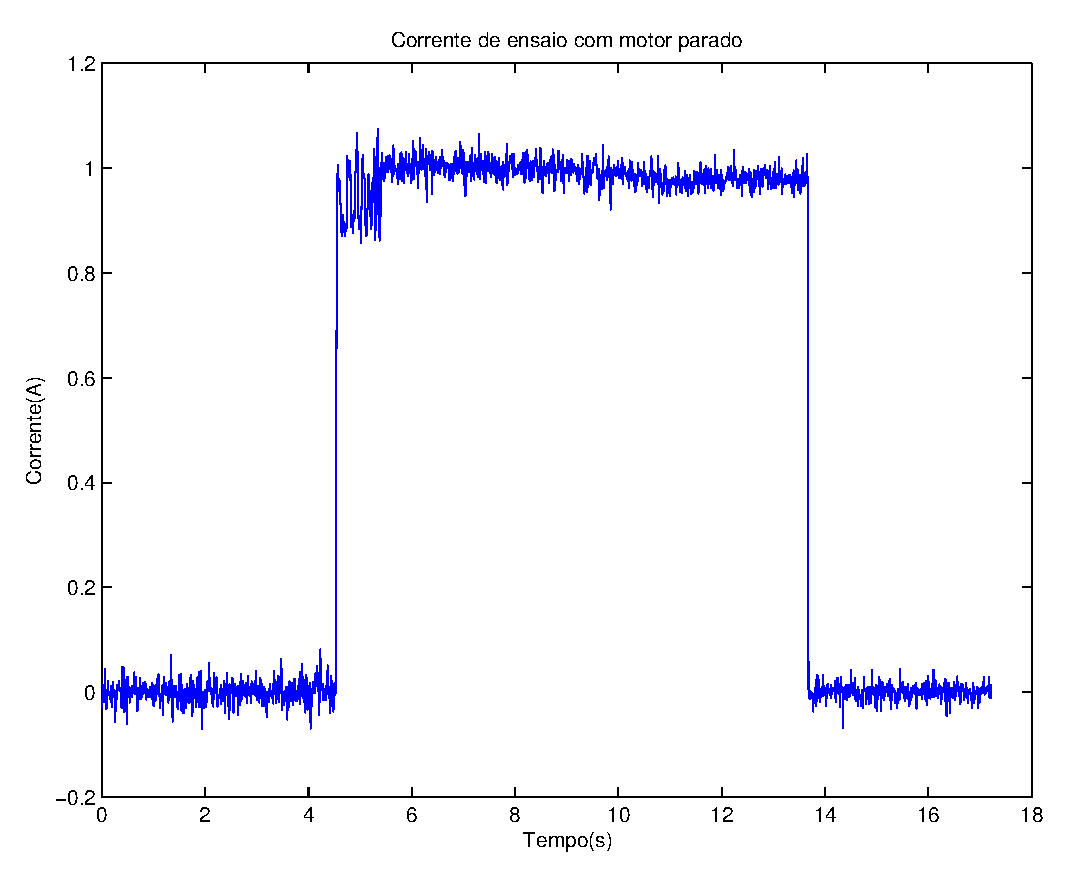
\includegraphics[height=0.4\linewidth]{ensaiop}
			}
		\end{center}
	\end{block}
\end{frame}
%------------------------------------------------
\begin{frame}
\frametitle{Determinação da Planta}
\begin{columns}
	\begin{column}{0.5\textwidth}
	\begin{block}{Ensaio com o motor livre}
		Analisar o comportamento do motor
		\begin{center}
			\resizebox{0.8\textwidth}{!}{%
				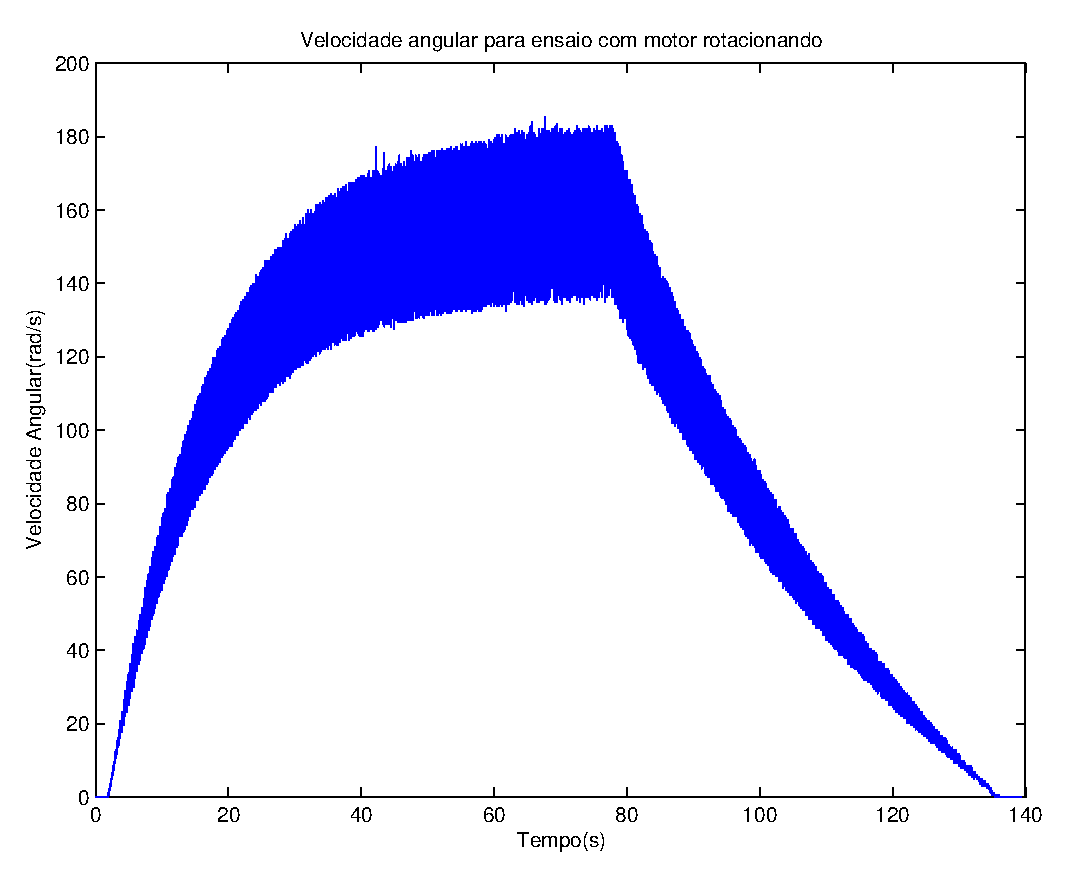
\includegraphics[height=0.4\linewidth]{ensaiorv}
				\quad
				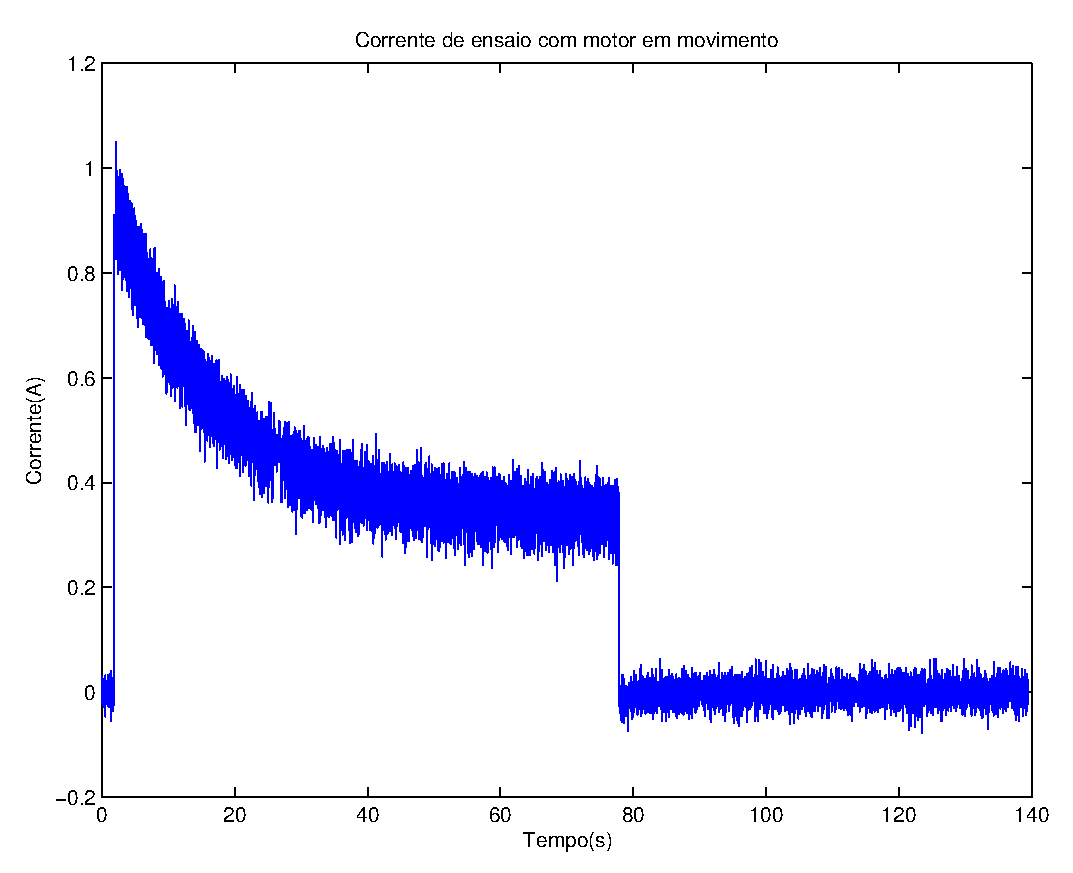
\includegraphics[height=0.4\linewidth]{ensaiori}
			}
		\end{center}
	\end{block}
	\end{column}
	
	\begin{column}{0.5\textwidth}
	\begin{block}{Ensaio com o motor desligado}
		Analisar o comportamento dos discos e da mola
		
		
		\begin{center}
			\resizebox{\textwidth}{!}{%
				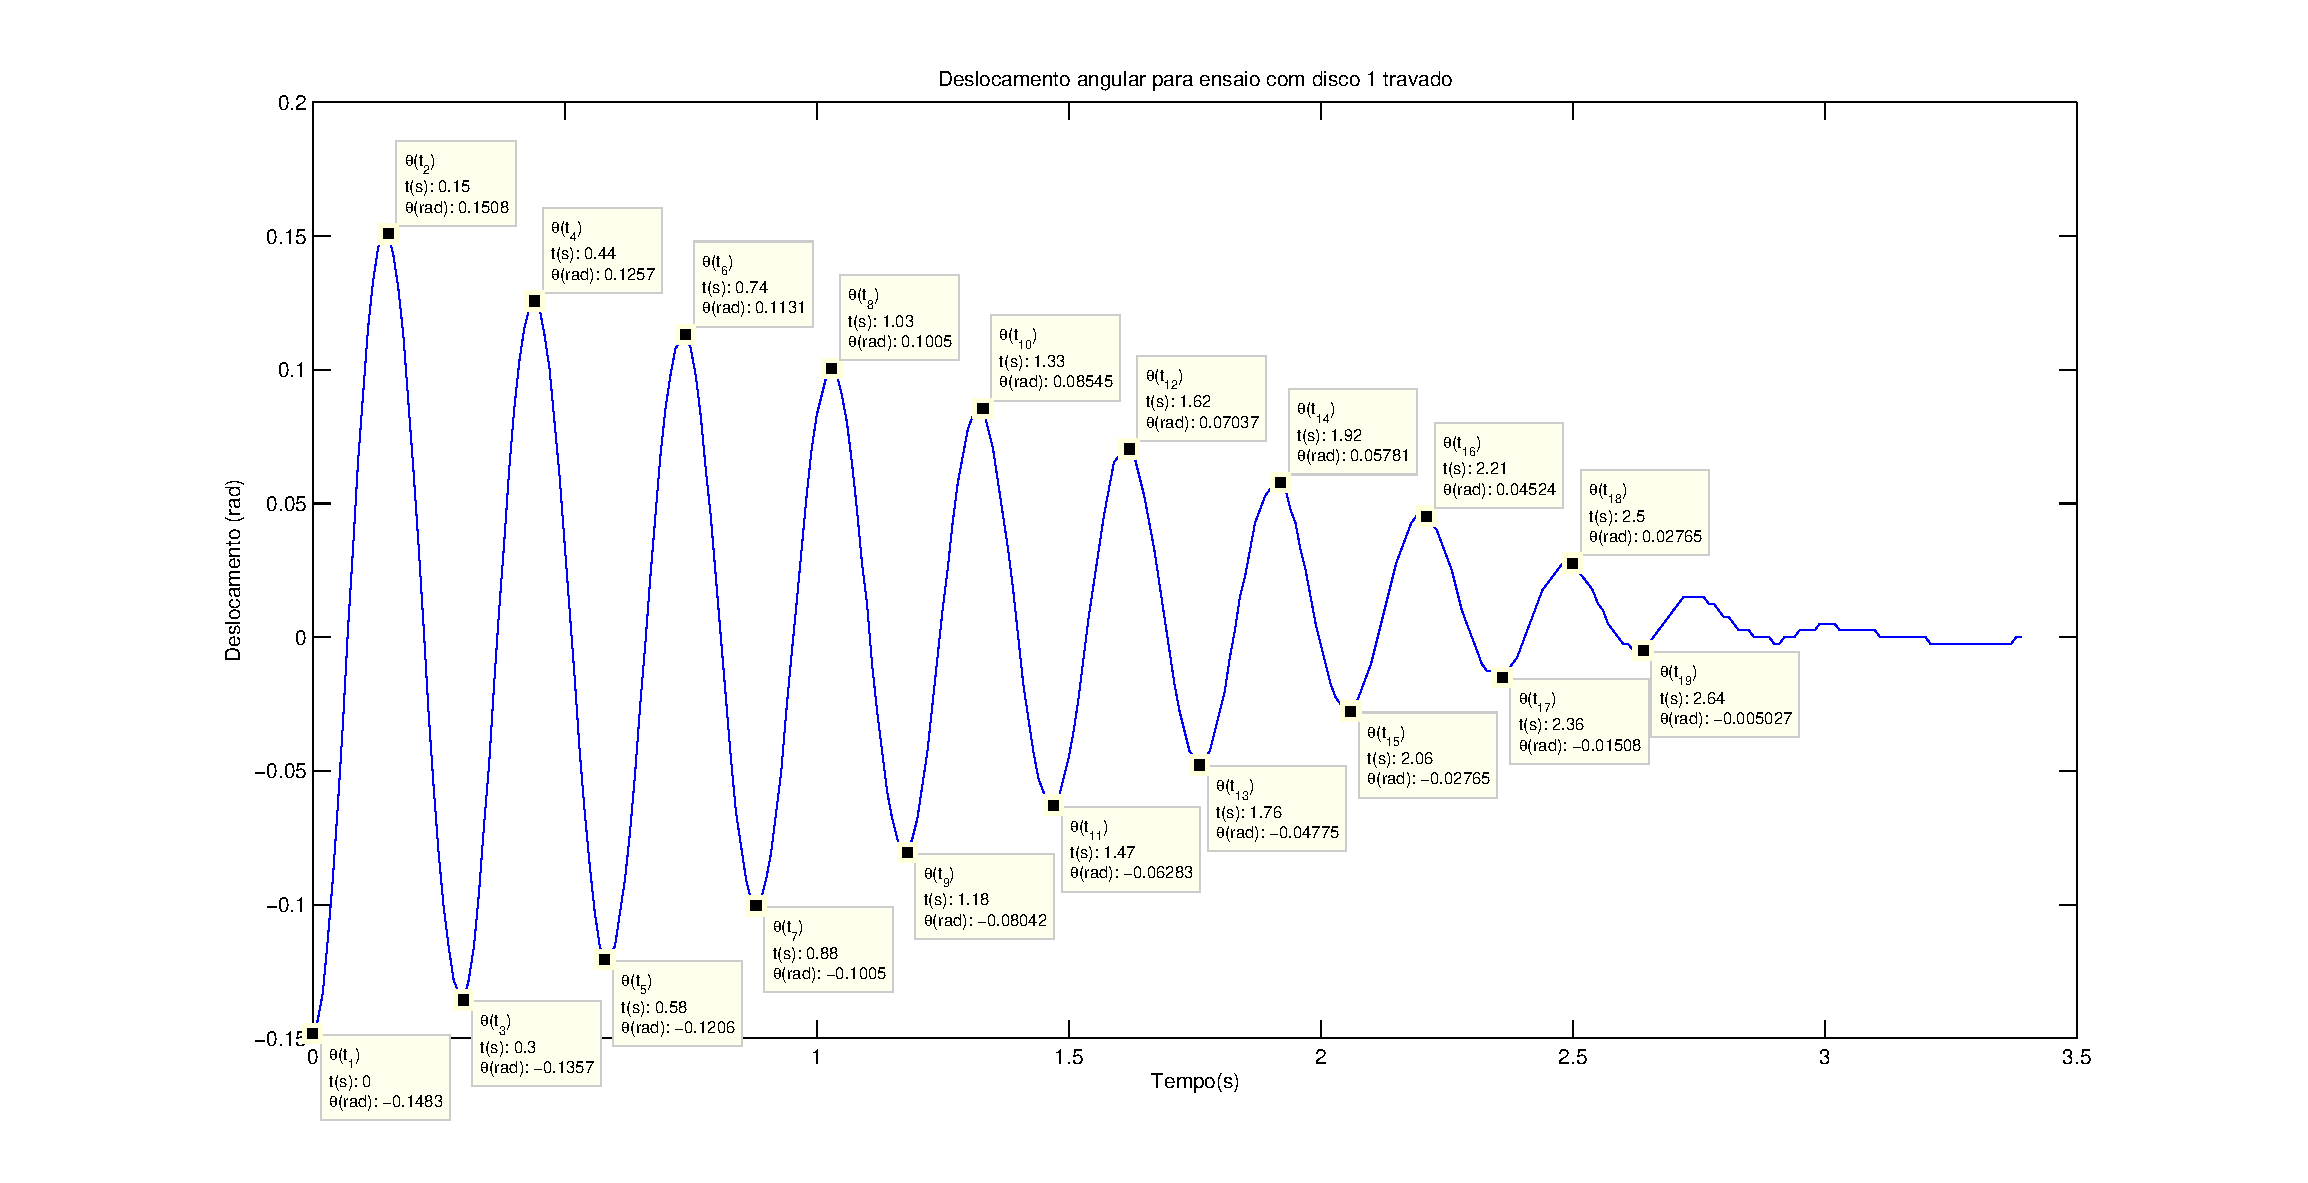
\includegraphics[height=0.5\linewidth]{disco1travado}
				\quad
				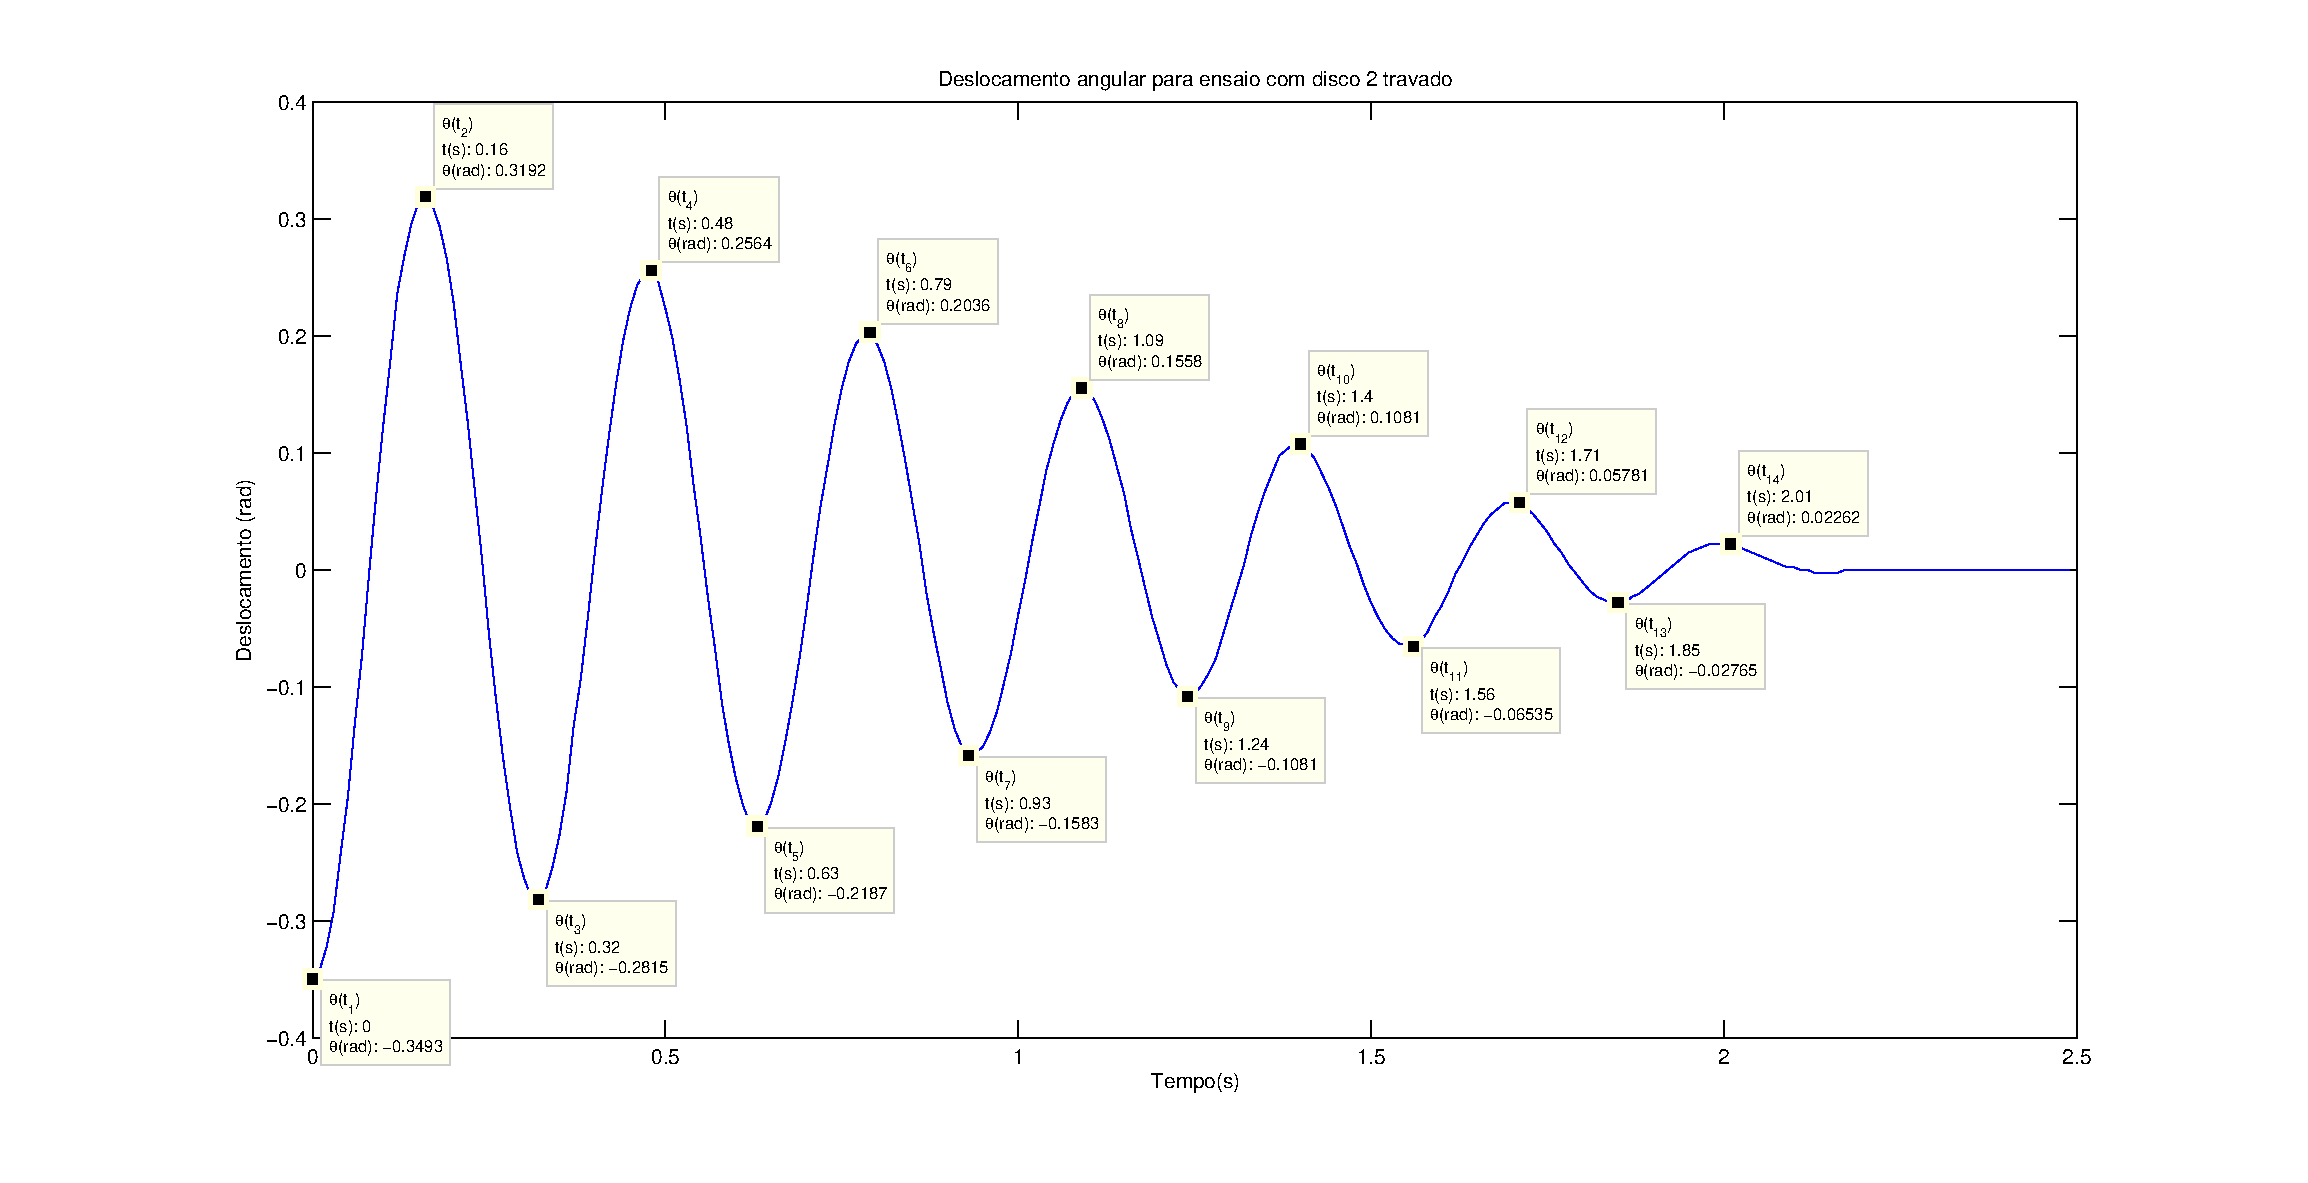
\includegraphics[height=0.5\linewidth]{disco2travado}
			}
		\end{center}
	\end{block}
	\end{column}
\end{columns}
\end{frame}
%------------------------------------------------
\begin{frame}
\frametitle{Determinação da Planta}
\begin{block}{Parâmetros}
	\begin{table}[H]
		\centering
		\scalebox{0.7}{
		\begin{tabular}{|c|c|c|}
			\hline Parâmetro & Significado & Valor \\ 
			\hline $J_1$ & Momento de inércia do disco 1 & $4.1188\cdot10^{-4}kg\cdot m^2$\\ 
			\hline $J_2$ & Momento de inércia do disco 2 & $3.7095\cdot10^{-4}kg\cdot m^2$\\
			\hline $b_1$ & Coeficiente de amortecimento do disco 1 & $4.2052\cdot10^{-5}N\cdot m\cdot s$\\
			\hline $b_2$ & Coeficiente de amortecimento do disco 2 & $9.5110\cdot10^{-4}N\cdot m\cdot s$\\ 	 
			\hline $\kappa$ & Constante elástica da mola & $0.1708N\cdot m/rad$\\ 
			\hline $V$ & Tensão no motor & $12V$\\ 
			\hline $K$ & Constante mecânica do motor & $0.0663 V \cdot s$\\ 
			\hline $R$ & Resistência do motor e da medida& $4.0709\Omega$ \\
			\hline $L$ & Indutância do motor & $0H$ \\ 	
			\hline 
		\end{tabular}
		} 
	\end{table}
\end{block}
\end{frame}

%------------------------------------------------
\begin{frame}
\frametitle{Determinação da Planta}
\begin{block}{Equação de Estados}
	\begin{equation*}
	\label{eq:ss}
	\left[ \begin{array}{c}
	\dot{x_1} \\
	\dot{x_2} \\
	\dot{x_3} \end{array} \right]
	=
	\left[ \begin{array}{ccc}
	0 & 1 & -1 \\
	-\frac{\kappa}{J_1} & -\frac{(b_1+K^2/R)}{J_1} & 0 \\
	\frac{\kappa}{J_2} & 0 & -\frac{b_2}{J_2} \end{array} \right]
	\left[ \begin{array}{c}
	x_1 \\
	x_2 \\
	x_3  \end{array} \right]
	+
	\left[ \begin{array}{c}
	0 				\\
	\frac{K}{RJ_1} 	\\
	0				\end{array} \right]
	V
	\end{equation*}
	\begin{equation*}
	\label{eq:ssval}
	\left[ \begin{array}{c}
	\dot{x_1} \\
	\dot{x_2} \\
	\dot{x_3} \end{array} \right]
	=
	\left[ \begin{array}{ccc}
	0 & 1 & -1 \\
	-414.71 & -2.73 & 0 \\
	-460.46 & 0 & -2.56 \end{array} \right]
	\left[ \begin{array}{c}
	x_1 \\
	x_2 \\
	x_3  \end{array} \right]
	+
	\left[ \begin{array}{c}
	0 				\\
	39.54 	\\
	0				\end{array} \right]
	V
	\end{equation*}
\end{block}
\end{frame}
%------------------------------------------------
\begin{frame}
\frametitle{Simulação}
\begin{figure}
	\centering
	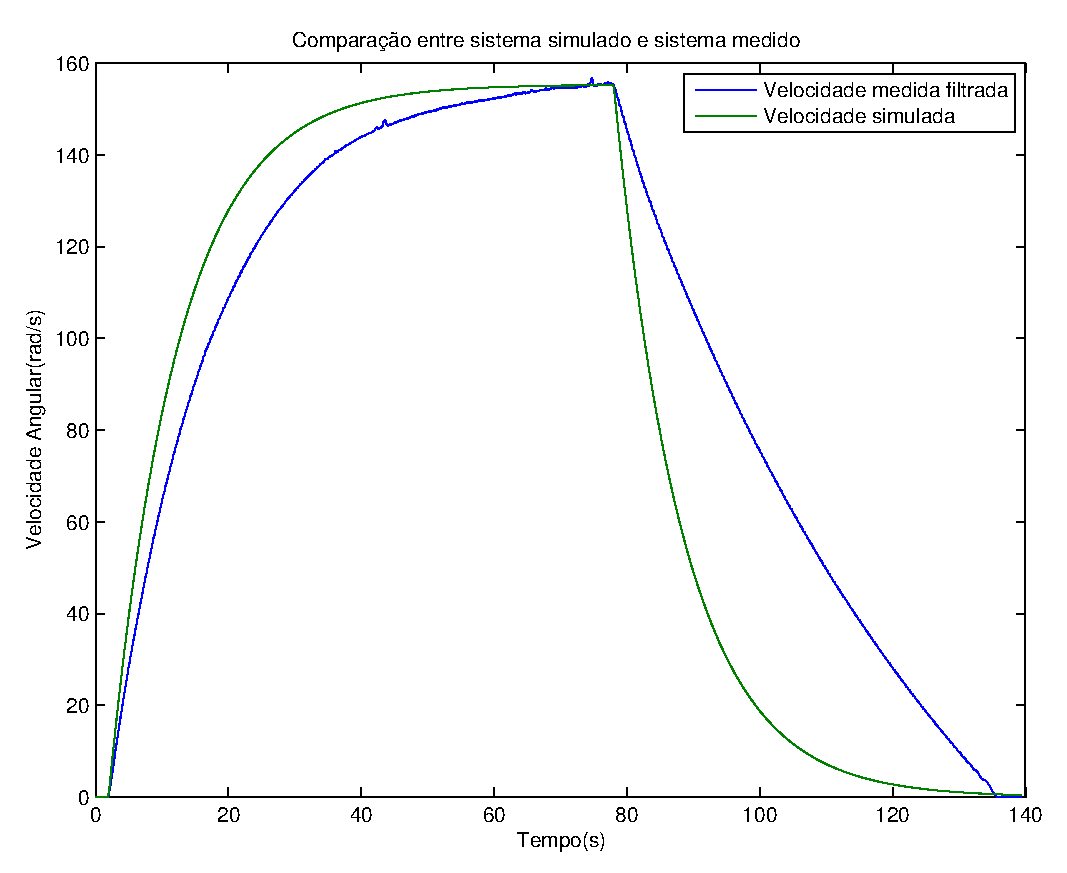
\includegraphics[width=0.7\linewidth]{simv}
\end{figure}
\end{frame}

%------------------------------------------------
\subsection{Controlador PI}
\begin{frame}
	\frametitle{Controlador PI}
	Modelo da planta pouco confiável, robustez desejada.
	\begin{equation*}
	K(s) = \kappa_p + \frac{\kappa_i}{s} = 0.097 + \frac{0.229}{s}
	\end{equation*}
	\begin{figure}
		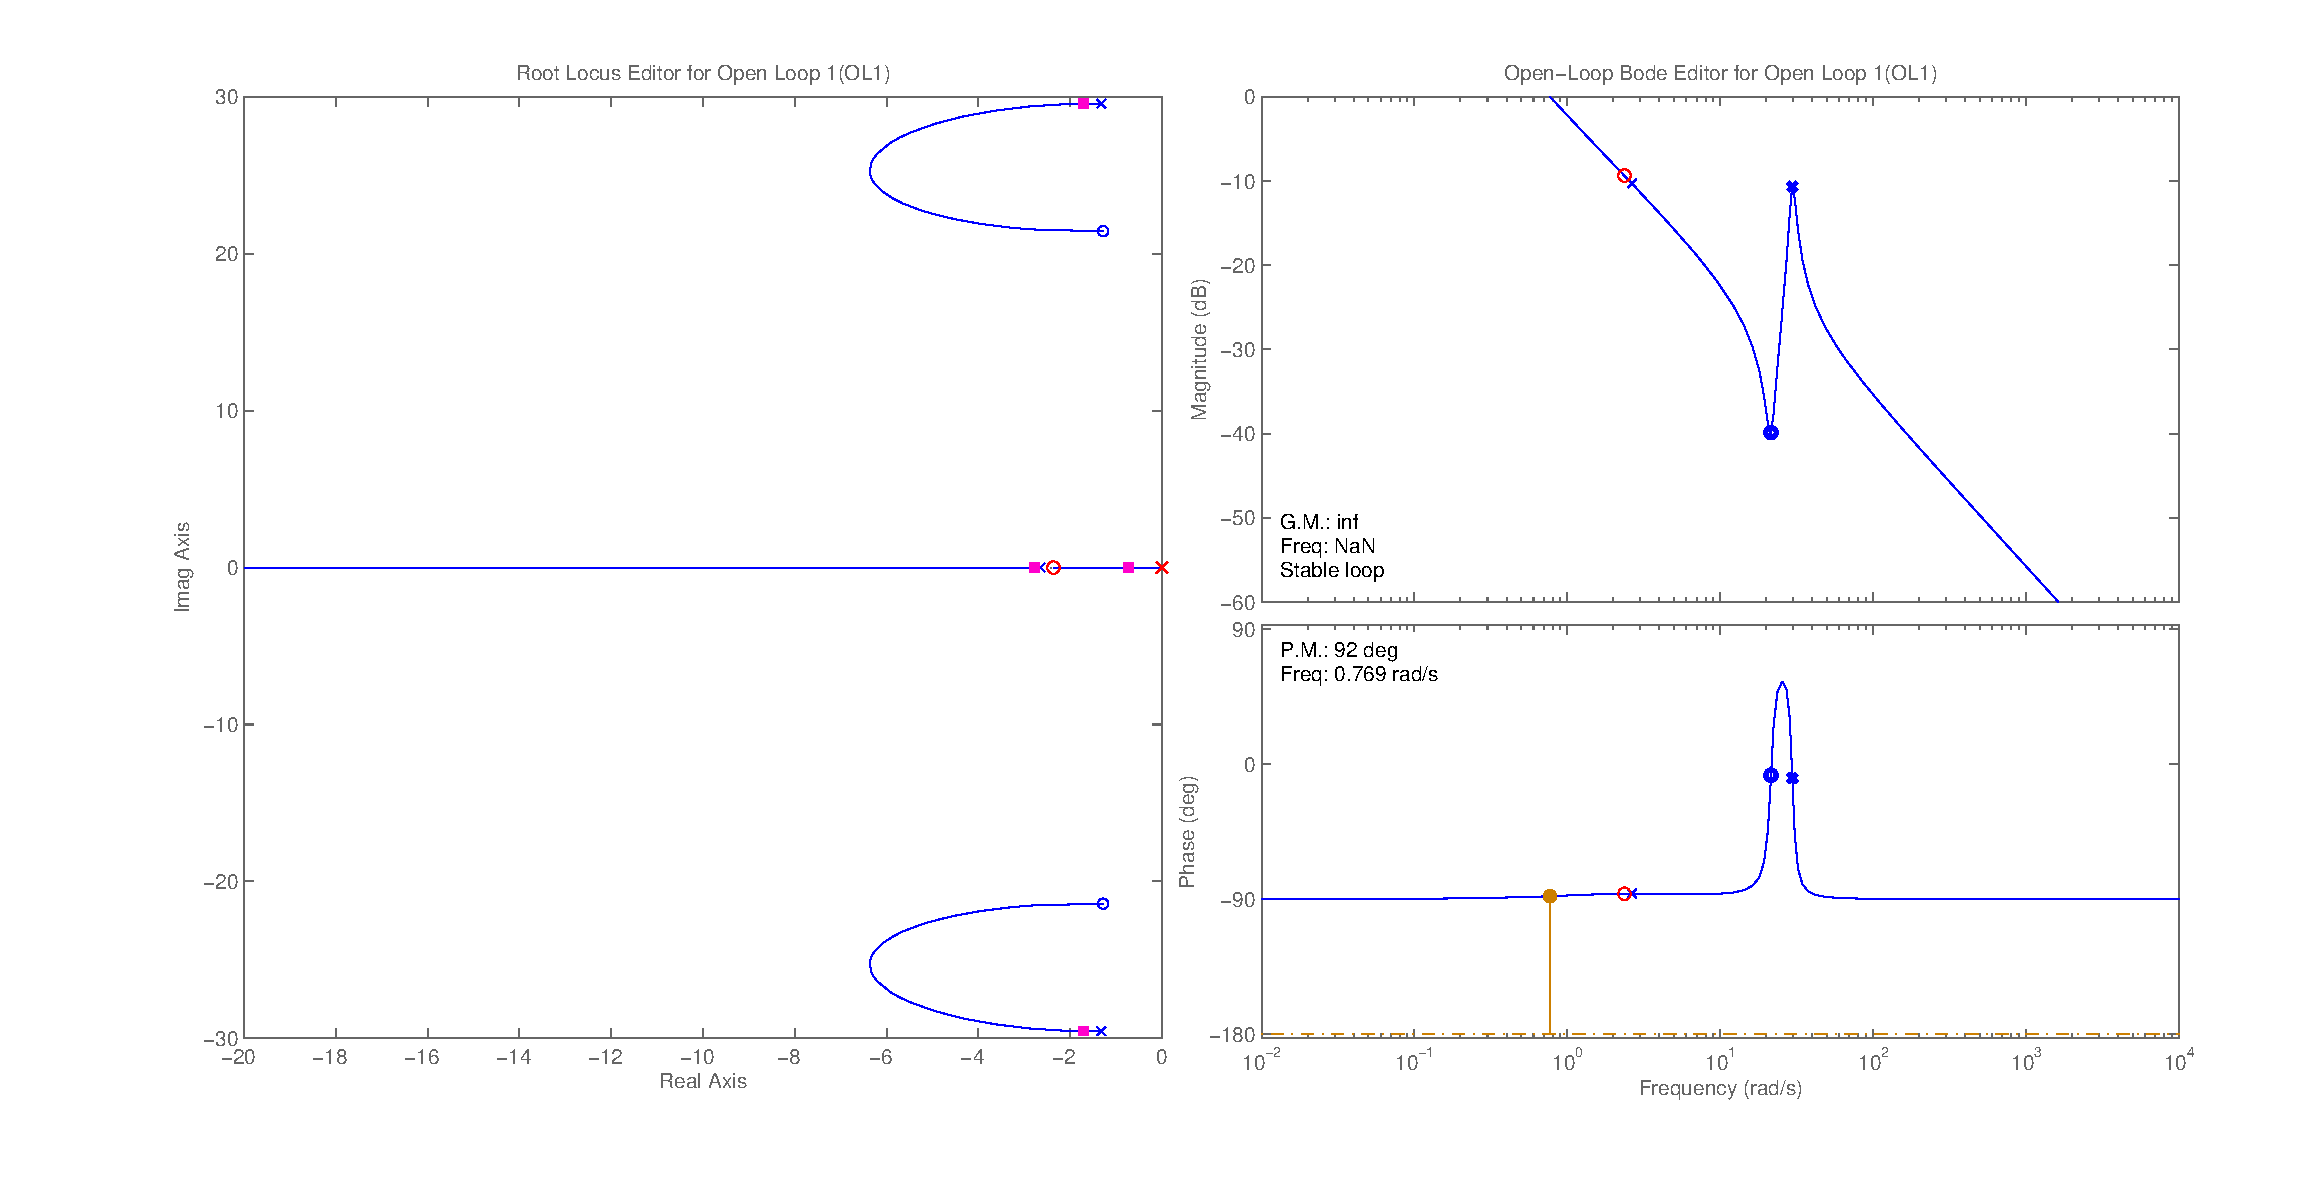
\includegraphics[height=0.4\linewidth]{../sisotool}
	\end{figure}
\end{frame}
%------------------------------------------------
\begin{frame}
	\frametitle{Simulação}
	\begin{figure}
		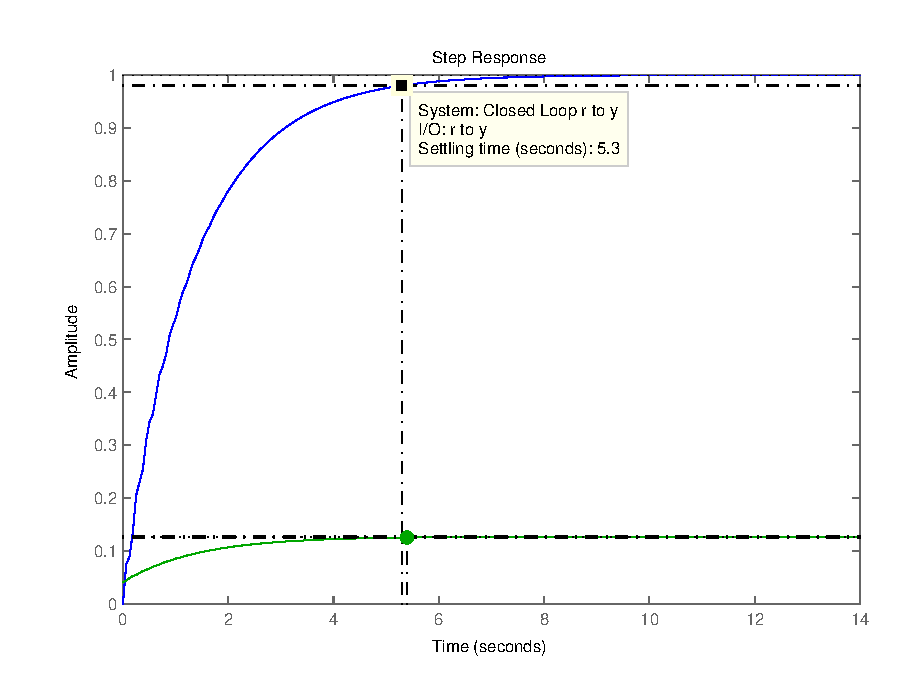
\includegraphics[height=0.6\linewidth]{../bla}
	\end{figure}
\end{frame}
%------------------------------------------------
\section{Teste de controle}
\begin{frame}
	\frametitle{Teste de controle}
		\begin{center}
			\resizebox{\textwidth}{!}{%
				\includegraphics[height=0.6\linewidth]{../blamedido}
				\quad
				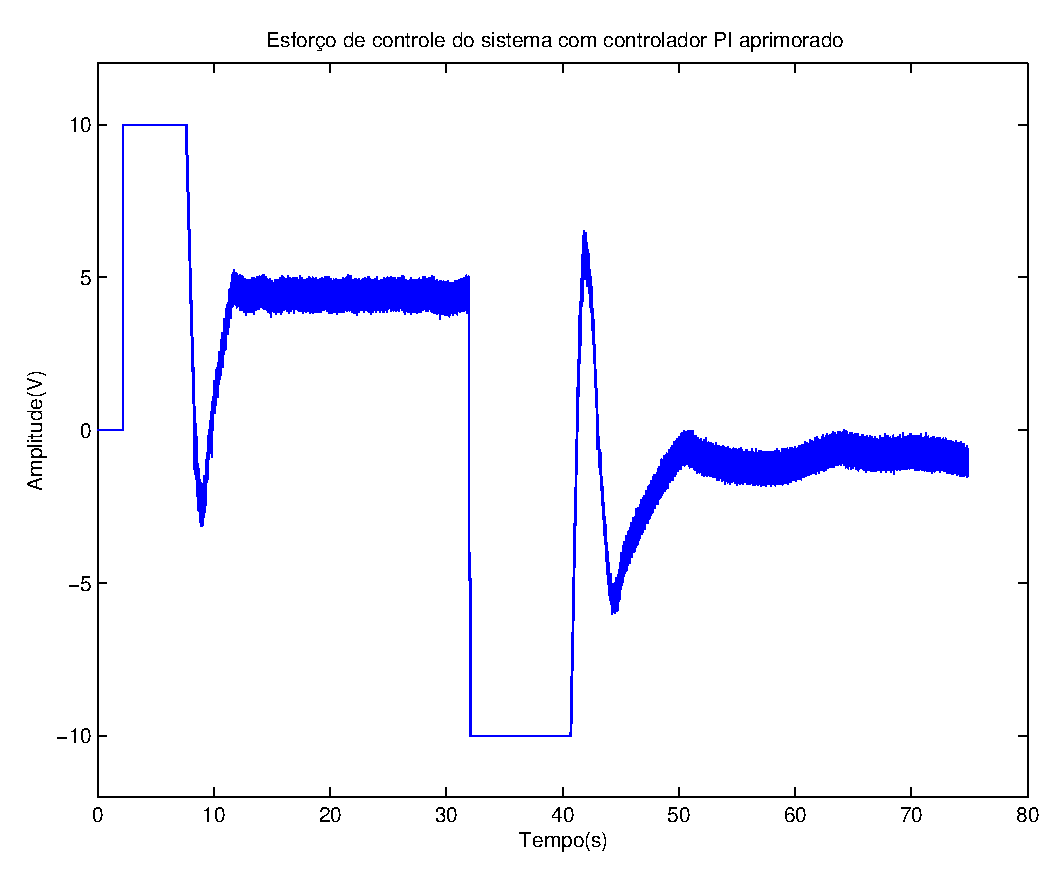
\includegraphics[height=0.6\linewidth]{../blaesforco}
			}
		\end{center}
\end{frame}
%------------------------------------------------
\begin{frame}
	\frametitle{Teste de controle}
	\begin{block}{Novo controlador PI}
		\begin{center}
			\scalebox{0.7}{ %
				$K(s) = \kappa_p + \frac{\kappa_i}{s} = 0.1 + \frac{0.1}{s}$
			}
			\begin{center}
				\includegraphics[width=0.4\linewidth]{../bla0101}
			\end{center}
		\end{center}

	\end{block}
\end{frame}
\section{Comentários finais}
%TODO Concluir que a Grace é escrota
\section{Perguntas}
\begin{frame}
\Huge{\centerline{Perguntas?}}
\end{frame}

%----------------------------------------------------------------------------------------

\end{document} 